% Copyright 2007 by Till Tantau
%
% This file may be distributed and/or modified
%
% 1. under the LaTeX Project Public License and/or
% 2. under the GNU Public License.
%
% See the file doc/licenses/LICENSE for more details.



\documentclass{beamer}

%
% DO NOT USE THIS FILE AS A TEMPLATE FOR YOUR OWN TALKS�!!
%
% Use a file in the directory solutions instead.
% They are much better suited.
%


% Setup appearance:

\usetheme{Darmstadt}
\usefonttheme[onlylarge]{structurebold}
\setbeamerfont*{frametitle}{size=\normalsize,series=\bfseries}
\setbeamertemplate{navigation symbols}{}


% Standard packages

\usepackage[english]{babel}
\usepackage[latin1]{inputenc}
\usepackage{times}
\usepackage[T1]{fontenc}

% Setup TikZ

\usepackage{tikz}
\usetikzlibrary{arrows}
\tikzstyle{block}=[draw opacity=0.7,line width=1.4cm]

% Setup pygments
\usepackage{fancyvrb}
\usepackage{color}

\newcommand\at{@}
\newcommand\lb{[}
\newcommand\rb{]}
\newcommand\PYbg[1]{\textcolor[rgb]{0.00,0.50,0.00}{\textbf{#1}}}
\newcommand\PYbf[1]{\textcolor[rgb]{0.73,0.40,0.53}{\textbf{#1}}}
\newcommand\PYbe[1]{\textcolor[rgb]{0.40,0.40,0.40}{#1}}
\newcommand\PYbd[1]{\textcolor[rgb]{0.73,0.13,0.13}{#1}}
\newcommand\PYbc[1]{\textcolor[rgb]{0.00,0.50,0.00}{\textbf{#1}}}
\newcommand\PYbb[1]{\textcolor[rgb]{0.40,0.40,0.40}{#1}}
\newcommand\PYba[1]{\textcolor[rgb]{0.00,0.00,0.50}{\textbf{#1}}}
\newcommand\PYaJ[1]{\textcolor[rgb]{0.73,0.13,0.13}{#1}}
\newcommand\PYaK[1]{\textcolor[rgb]{0.00,0.00,1.00}{#1}}
\newcommand\PYaH[1]{\fcolorbox[rgb]{1.00,0.00,0.00}{1,1,1}{#1}}
\newcommand\PYaI[1]{\textcolor[rgb]{0.69,0.00,0.25}{#1}}
\newcommand\PYaN[1]{\textcolor[rgb]{0.00,0.00,1.00}{\textbf{#1}}}
\newcommand\PYaO[1]{\textcolor[rgb]{0.00,0.00,0.50}{\textbf{#1}}}
\newcommand\PYaL[1]{\textcolor[rgb]{0.73,0.73,0.73}{#1}}
\newcommand\PYaM[1]{\textcolor[rgb]{0.74,0.48,0.00}{#1}}
\newcommand\PYaB[1]{\textcolor[rgb]{0.00,0.25,0.82}{#1}}
\newcommand\PYaC[1]{\textcolor[rgb]{0.67,0.13,1.00}{#1}}
\newcommand\PYaA[1]{\textcolor[rgb]{0.00,0.50,0.00}{#1}}
\newcommand\PYaF[1]{\textcolor[rgb]{1.00,0.00,0.00}{#1}}
\newcommand\PYaG[1]{\textcolor[rgb]{0.10,0.09,0.49}{#1}}
\newcommand\PYaD[1]{\textcolor[rgb]{0.25,0.50,0.50}{\textit{#1}}}
\newcommand\PYaE[1]{\textcolor[rgb]{0.63,0.00,0.00}{#1}}
\newcommand\PYaZ[1]{\textcolor[rgb]{0.00,0.50,0.00}{\textbf{#1}}}
\newcommand\PYaX[1]{\textcolor[rgb]{0.00,0.50,0.00}{#1}}
\newcommand\PYaY[1]{\textcolor[rgb]{0.73,0.13,0.13}{#1}}
\newcommand\PYaR[1]{\textcolor[rgb]{0.10,0.09,0.49}{#1}}
\newcommand\PYaS[1]{\textcolor[rgb]{0.25,0.50,0.50}{\textit{#1}}}
\newcommand\PYaP[1]{\textcolor[rgb]{0.49,0.56,0.16}{#1}}
\newcommand\PYaQ[1]{\textcolor[rgb]{0.40,0.40,0.40}{#1}}
\newcommand\PYaV[1]{\textcolor[rgb]{0.00,0.00,1.00}{\textbf{#1}}}
\newcommand\PYaW[1]{\textcolor[rgb]{0.73,0.13,0.13}{#1}}
\newcommand\PYaT[1]{\textcolor[rgb]{0.50,0.00,0.50}{\textbf{#1}}}
\newcommand\PYaU[1]{\textcolor[rgb]{0.82,0.25,0.23}{\textbf{#1}}}
\newcommand\PYaj[1]{\textcolor[rgb]{0.00,0.50,0.00}{#1}}
\newcommand\PYak[1]{\textcolor[rgb]{0.73,0.40,0.53}{#1}}
\newcommand\PYah[1]{\textcolor[rgb]{0.63,0.63,0.00}{#1}}
\newcommand\PYai[1]{\textcolor[rgb]{0.10,0.09,0.49}{#1}}
\newcommand\PYan[1]{\textcolor[rgb]{0.67,0.13,1.00}{\textbf{#1}}}
\newcommand\PYao[1]{\textcolor[rgb]{0.73,0.40,0.13}{\textbf{#1}}}
\newcommand\PYal[1]{\textcolor[rgb]{0.25,0.50,0.50}{\textit{#1}}}
\newcommand\PYam[1]{\textbf{#1}}
\newcommand\PYab[1]{\textit{#1}}
\newcommand\PYac[1]{\textcolor[rgb]{0.73,0.13,0.13}{#1}}
\newcommand\PYaa[1]{\textcolor[rgb]{0.50,0.50,0.50}{#1}}
\newcommand\PYaf[1]{\textcolor[rgb]{0.25,0.50,0.50}{\textit{#1}}}
\newcommand\PYag[1]{\textcolor[rgb]{0.40,0.40,0.40}{#1}}
\newcommand\PYad[1]{\textcolor[rgb]{0.73,0.13,0.13}{#1}}
\newcommand\PYae[1]{\textcolor[rgb]{0.40,0.40,0.40}{#1}}
\newcommand\PYaz[1]{\textcolor[rgb]{0.00,0.63,0.00}{#1}}
\newcommand\PYax[1]{\textcolor[rgb]{0.60,0.60,0.60}{\textbf{#1}}}
\newcommand\PYay[1]{\textcolor[rgb]{0.00,0.50,0.00}{\textbf{#1}}}
\newcommand\PYar[1]{\textcolor[rgb]{0.10,0.09,0.49}{#1}}
\newcommand\PYas[1]{\textcolor[rgb]{0.73,0.13,0.13}{\textit{#1}}}
\newcommand\PYap[1]{\textcolor[rgb]{0.00,0.50,0.00}{#1}}
\newcommand\PYaq[1]{\textcolor[rgb]{0.53,0.00,0.00}{#1}}
\newcommand\PYav[1]{\textcolor[rgb]{0.00,0.50,0.00}{\textbf{#1}}}
\newcommand\PYaw[1]{\textcolor[rgb]{0.40,0.40,0.40}{#1}}
\newcommand\PYat[1]{\textcolor[rgb]{0.10,0.09,0.49}{#1}}
\newcommand\PYau[1]{\textcolor[rgb]{0.40,0.40,0.40}{#1}}

%pygmentize -f latex hello.py
%\begin{frame}[fragile]
%\begin{Verbatim}[commandchars=@\[\]]
%@PYaD[#!/usr/bin/env python]
%@PYay[print] @PYad["]@PYad[hello]@PYad["]
%\end{Verbatim}


% Author, Title, etc.

\title[Experimentation with python - why not do it the FOSS way?] 
{%
  \textbf{Experimentation with python} \\ \textit{Why not do it the FOSS way?}%
}

\author[Suryajith, Praneeth]
{
  Suryajith Chillara\inst{1} \and
  Praneeth Bodduluri\inst{1}
}

\institute[IIT Kanpur]
{
  \inst{1}%
  Indian Institute of Technology, Kanpur
}

\date[SciPy.in 2009]
{SciPy India Conference, 2009}



% The main document

\begin{document}

\begin{frame}
  \titlepage
\end{frame}

\begin{frame}{Outline}
  \tableofcontents
\end{frame}


\section{Introduction}


\begin{frame}[fragile]{Current state of instrumentation software} 
  You hopefully know this after the previous three talks\dots



\end{frame}

\begin{frame}[t]{General formalization of haplotyping.}
  \begin{block}{Inputs}
    \begin{itemize}
    \item A \alert{genotype matrix} $G$.
    \item The \alert{rows} of the matrix are \alert{taxa / individuals}.
    \item The \alert{columns} of the matrix are \alert{SNP sites /
        characters}. 
    \end{itemize}
  \end{block}
  \begin{block}{Outputs}
    \begin{itemize}
    \item A \alert{haplotype matrix} $H$.
    \item Pairs of rows in $H$ \alert{explain} the rows of $G$.
    \item The haplotypes in $H$ are \alert{biologically plausible}. 
    \end{itemize}
  \end{block}
\end{frame}



\section*{Summary}

\begin{frame}
  \frametitle<presentation>{Summary}

  \begin{itemize}
  \item
    Finding optimal pp-partitions is \alert{intractable}. 
  \item
    It is even intractable to find a pp-partition when \alert{just two 
      noncontiguous  blocks are known to suffice}.
  \item
    For perfect \alert{path} phylogenies, optimal partitions can be
    computed \alert{in polynomial time}.
  \end{itemize}
\end{frame}


\appendix

\section*{Appendix}

\begin{frame}[label=algorithm]{The algorithm in action.}{Computation of
    the partial order.}
  \begin{columns}[t]
    \column{.4\textwidth}
    \begin{exampleblock}{Genotype matrix}
      $G\colon$
      \begin{tabular}{ccccc}
        A & B & C & D & E \\\hline
        2 & 2 & 2 & 2 & 2 \\
        0 & 1 & 2 & 1 & 0 \\
        1 & 0 & 0 & 1 & 2 \\
        0 & 2 & 2 & 0 & 0
      \end{tabular}
    \end{exampleblock}
    \column{.6\textwidth}
    \begin{exampleblock}{Partial order}
      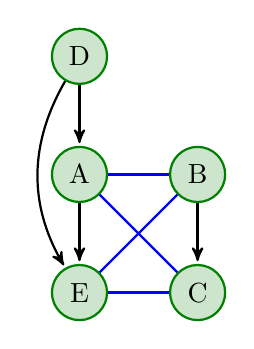
\begin{tikzpicture}[node distance=15mm]
        \tikzstyle{every node}=
        [%
          fill=green!50!black!20,%
          draw=green!50!black,%
          minimum size=7mm,%
          circle,%
          thick%
        ]

        \node (A) {A};
        \node (B) [right of=A] {B};
        \node (C) [below of=B] {C};
        \node (D) [above of=A] {D};
        \node (E) [below of=A] {E};

        \path [thick,shorten >=1pt,-stealth'] (A) edge (E)
                         (B) edge (C)
                         (D) edge (A)
                             edge[bend right] (E);

        \uncover<2>{
        \path [-,blue,thick](A) edge (B)
                                edge (C)  
                            (B) edge (E)
                            (C) edge (E);}
      \end{tikzpicture}

      Partial order: \tikz[baseline] \draw[thick,-stealth'] (0pt,.5ex)
      -- (5mm,.5ex); 

      \uncover<2>{\textcolor{blue}{Compatible as children of root:
          \tikz[baseline] \draw[thick] (0pt,.5ex) -- (5mm,.5ex);}} 
    \end{exampleblock}
  \end{columns}  
\end{frame}

\begin{frame}{The algorithm in action.}{The matching in the special graph.}
  \begin{columns}[t]
    \column{.3\textwidth}
    \begin{exampleblock}{Partial order}
      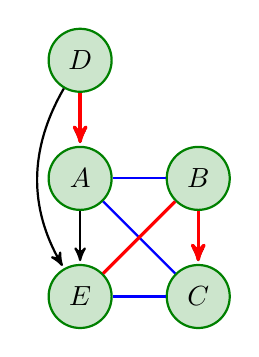
\begin{tikzpicture}[node distance=15mm]
        \tikzstyle{every node}=%
        [%
          fill=green!50!black!20,%
          draw=green!50!black,%
          minimum size=8mm,%
          circle,%
          thick%
        ]

        \node (A)              {$A$};
        \node (B) [right of=A] {$B$};
        \node (C) [below of=B] {$C$};
        \node (D) [above of=A] {$D$};
        \node (E) [below of=A] {$E$};

        \path [thick,shorten >=1pt,-stealth'] (A) edge (E)
                         (B) edge (C)
                         (D) edge (A)
                             edge[bend right] (E);

        \path [-,blue,thick](A) edge (B)
                                edge (C)  
                            (B) edge (E)
                            (C) edge (E);

        \only<3->
        {
          \path[very thick,shorten >=1pt,-stealth',red] (D) edge (A) (B) edge (C);
          \path [-,red,very thick](E) edge (B);
        }
      \end{tikzpicture}
    \end{exampleblock}
    \column{.7\textwidth}
    \begin{exampleblock}{Matching graph}
      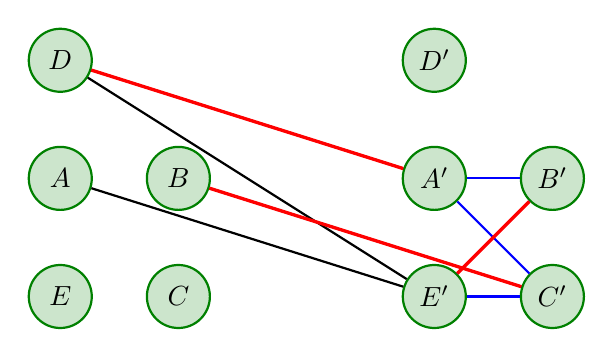
\begin{tikzpicture}[node distance=15mm]
        \tikzstyle{every node}=%
        [%
          fill=green!50!black!20,%
          draw=green!50!black,%
          minimum size=8mm,%
          circle,%
          thick,%
          inner sep=0pt%
        ]

        \node (A)              {$A$};
        \node (B) [right of=A] {$B$};
        \node (C) [below of=B] {$C$};
        \node (D) [above of=A] {$D$};
        \node (E) [below of=A] {$E$};

        \begin{scope}[xshift=4.75cm]
          \node (A')               {$A'$};
          \node (B') [right of=A'] {$B'$};
          \node (C') [below of=B'] {$C'$};
          \node (D') [above of=A'] {$D'$};
          \node (E') [below of=A'] {$E'$};
        \end{scope}
        
        \path [thick]    (A) edge (E')
                         (B) edge (C')
                         (D) edge (A')
                             edge (E');

        \path [blue,thick](A') edge (B')
                               edge (C')  
                          (B') edge (E')
                          (C') edge (E');

        \only<2->
        {
          \path[very thick,red] (D) edge (A')
                           (B) edge (C')
                           (B') edge (E');
        }
      \end{tikzpicture}
    \end{exampleblock}
  \end{columns}

  \medskip
  \uncover<2->{A \alert{maximal matching} in the matching graph
    \uncover<3>{induces\\ \alert{perfect path phylogenies}.}}

  \hfill\hyperlink{return}{\beamerreturnbutton{Return}}
\end{frame}

\end{document}


